\documentclass[12pt,a4paper, xcolor=table]{article}
\usepackage{graphicx}
\usepackage[utf8]{inputenc}
\usepackage{eurosym}
\usepackage[spanish,es-tabla]{babel}
\usepackage[left=2cm, right=2cm, top=2cm, bottom=2cm]{geometry}
\usepackage{afterpage}
\PassOptionsToPackage{hyphens}{url}\usepackage{hyperref}
\usepackage{subfig}
\usepackage[table,xcdraw]{xcolor}
\usepackage{cite}
\usepackage{url}
\usepackage{changepage}

\usepackage{imakeidx}
\newcommand\blankpage{%
    \null
    \thispagestyle{empty}%
    \addtocounter{page}{-1}%
    \newpage}
\renewcommand*\contentsname{Índice: }

\makeindex
\let\olditemize\itemize
\def\itemize{\olditemize\itemsep=0pt}

\begin{document}
\setlength{\parindent}{0pt}
\begin{titlepage}
        \centering
        
\includegraphics[width=0.75\textwidth]{img/logo_uc3m.jpg}\par\vspace{2cm}
        {\huge\bfseries Práctica Final \\ Predicción del género de libros\par}
        \vspace{0.5cm}
        {\scshape\Large Inteligencia Artificial en las Organizaciones\par}
        \vspace{1.5cm}
        {\scshape\Large Grupo 83-1\par}
        \vspace{1.5cm}
        {\Large\itshape Miguel Gutiérrez Pérez\par}
        {\Large 100383537@alumnos.uc3m.es \par}
        \vspace{1cm}
        {\Large\itshape Mario Lozano Cortés\par}
        {\Large 100383511@alumnos.uc3m.es\par}
        \vspace{1cm}
        {\Large\itshape Alba Reinders Sánchez\par}
        {\Large 100383444@alumnos.uc3m.es\par}
        \vspace{1cm}
        {\Large\itshape Alejandro Valverde Mahou\par}
        {\Large 100383383@alumnos.uc3m.es\par}
        \vspace{5mm}
        {\large GitHub: \textbf{\textit{\href{https://github.com/Pheithar/InteligenciaArtificialOrganizaciones}{InteligenciaArtificialOrganizaciones}}}}
        \vfill

% Bottom of the page
        {\large \today\par}
\end{titlepage}

\tableofcontents

\newpage

\section{Introducción}

El objetivo de esta práctica consiste en abordar una clasificación sobre resúmenes de libros para determinar su género literario. Las razones que llevan a la elección de este problema tienen que ver con que actualmente cualquier persona con la dedicación suficiente puede escribir un libro sin la necesidad del patrocinio de una editorial, lo que conlleva una \textbf{explosión en el número de nuevos libros generados}. Por consiguiente, las librerías y bibliotecas necesitan catalogar una gran cantidad de escritos, lo cual, les lleva a necesitar de métodos de clasificación automática. Por ello, se plantea el uso de resúmenes y metadatos de los libros puesto que la tarea de clasificación \textbf{debe poder realizarse con el menor número de datos posible}, puesto que no todos los libros que llegan a estas entidades disponen de todos los datos completos.

\vspace{3mm}

La primera cuestión imprescindible que surge al conocer el problema propuesto es qué técnica de Inteligencia Artificial emplear. Dado que se realiza un análisis sobre diferentes textos, la opción evidente es la \textbf{Minería de Texto}, la cual es una técnica de minería de datos que busca extraer \textbf{información útil y relevante de documentos de texto} de diferentes fuentes diferentes, como puede ser páginas web,
correos electrónicos, periódicos o redes sociales. Para ello, se hace una identificación de patrones en los datos, como puede ser la repetición de palabras o conjuntos de palabras, estructuras sintácticas que se repitan a lo largo de los datos, etc. Esta minería de texto tiene numerosas aplicaciones, y en esta práctica se van a desarrollar una clasificación en función de unas categorías que serán definidas gracias a la elección de un dataset apropiado.

\vspace{3mm}

A continuación se ofrece un\textbf{ esquema del funcionamiento de la tarea propuesta }en donde un libro sin catalogación llega a alguna a de estas entidades que necesitan catalogar su género a partir de la información más reducida posible (generalmente título y argumento). Inicialmente se plantea la distinción de un único género, sin embargo, \textbf{es bien sabido que un escrito no tiene por qué adscribirse a un único género} y por lo tanto se debe considerar como futura \textbf{ampliación} catalogar tantos como sea posible.

\vspace{12mm}

  \begin{figure}[!h]
    \centering
    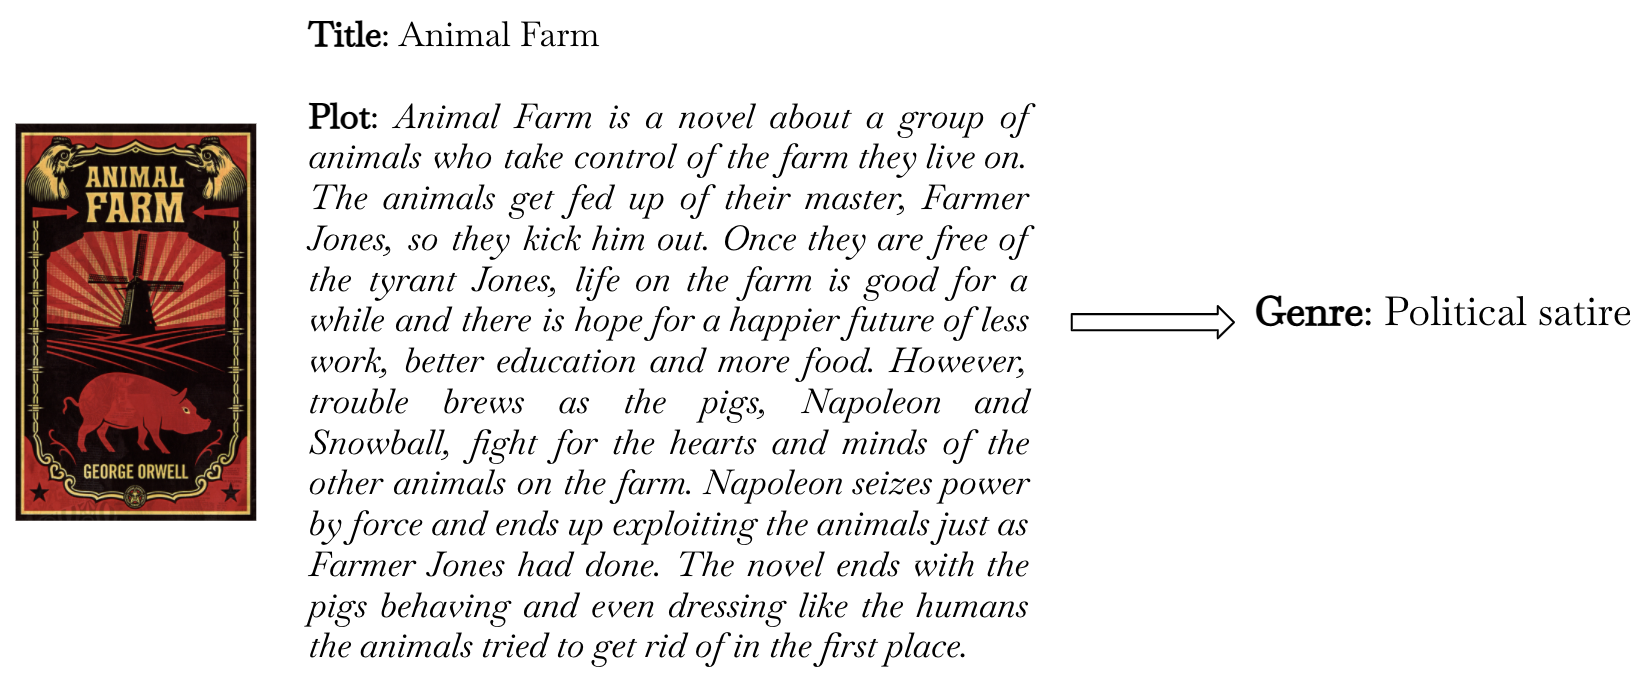
\includegraphics[width=450px]{img/Animal Farm.png}
    \caption{Esquema de la tarea}
    \end{figure}

\newpage

\section{Conceptos teóricos}

\section{Conclusiones}

\clearpage

\bibliographystyle{ieeetr}
\bibliography{bibliografia.bib}


\end{document}
